\documentclass[border=6pt]{standalone}
\usepackage{tikz}
\usepackage{pgfplots}
\pgfplotsset{compat=1.18}
\usetikzlibrary{arrows.meta,positioning,shapes.geometric,fit,backgrounds,calc,decorations.pathreplacing,patterns,pgfplots.groupplots}
\tikzset{
  blk/.style={rectangle, rounded corners=2pt, draw=black!70, thick, fill=blue!6,
              minimum height=8mm, minimum width=20mm, align=center, font=\small},
  io/.style={rectangle, rounded corners=6pt, draw=black!70, thick, fill=green!8,
             minimum height=8mm, align=center, font=\small},
  proc/.style={rectangle, draw=black!70, thick, fill=orange!10, minimum height=8mm,
               align=center, font=\small},
  dec/.style={diamond, aspect=2, draw=black!70, thick, fill=yellow!15, align=center, font=\footnotesize},
  warnbox/.style={rectangle, rounded corners=2pt, draw=red!60!black, thick, fill=red!7,
                  minimum height=8mm, align=center, font=\small},
  oklbox/.style={rectangle, rounded corners=2pt, draw=green!45!black, thick, fill=green!8,
                 minimum height=8mm, align=center, font=\small},
  ar/.style={-{Latex[length=2mm]}, thick},
  arl/.style={-{Latex[length=2mm]}, thick, dashed, draw=black!55},
  lbl/.style={font=\footnotesize\itshape, text=black!60},
  tag/.style={font=\tiny, inner sep=0.6pt, fill=white, fill opacity=0.85, text opacity=1},
  keyfont/.style={font=\fontsize{4.8}{5.7}\selectfont},
}
\definecolor{good}{RGB}{34,139,34}
\definecolor{bad}{RGB}{178,34,34}
\definecolor{warn}{RGB}{218,165,32}
\definecolor{pesblue}{RGB}{0,45,98}
\definecolor{complete}{RGB}{30,125,79}
\definecolor{partial}{RGB}{176,106,0}
\definecolor{blocked}{RGB}{166,43,43}
\begin{document}
% ---------------------------------------------------------------------------
% fig_scaling_null -- cross-scale GRPO reward vs. model scale (12 anchors,
% 4B-1T parameters).  NULL-RESULT FIGURE: shows the ABSENCE of a reliable
% monotone scaling trend.  No upward trend line is drawn anywhere.
%
% Data sources (real, read from repo):
%   platform_hybrid/experiments/results/scaling_law_extended_frontier.tsv
%       -> per-anchor params_B and r_mean (panel a); the remaining r_* columns
%          enter panel (b) only through the fitted slopes of the TSV below
%   platform_hybrid/experiments/results/scaling_law_power_law.tsv
%       -> OLS slope / se_slope / r2 / perm_p per metric, 12 anchors;
%          panel (b) error bars are 1.96 * se_slope (95% CI)
%   platform_hybrid/paper/sections/scaling_laws.tex (iter-25 audit)
%       -> per-step binomial noise floor sigma_step in [0.074, 0.119]
%       -> Spearman rho(log10 N, Rbar) = +0.149 (p = 0.64), 12 anchors
%       -> AICc selects the constant (intercept-only) model on all traces
%   Headroom note: panel (a) ymax extends to 1.78 so the statistics box sits
%   in an empty annotation band; no data point lies above y = 1.0.
% ---------------------------------------------------------------------------
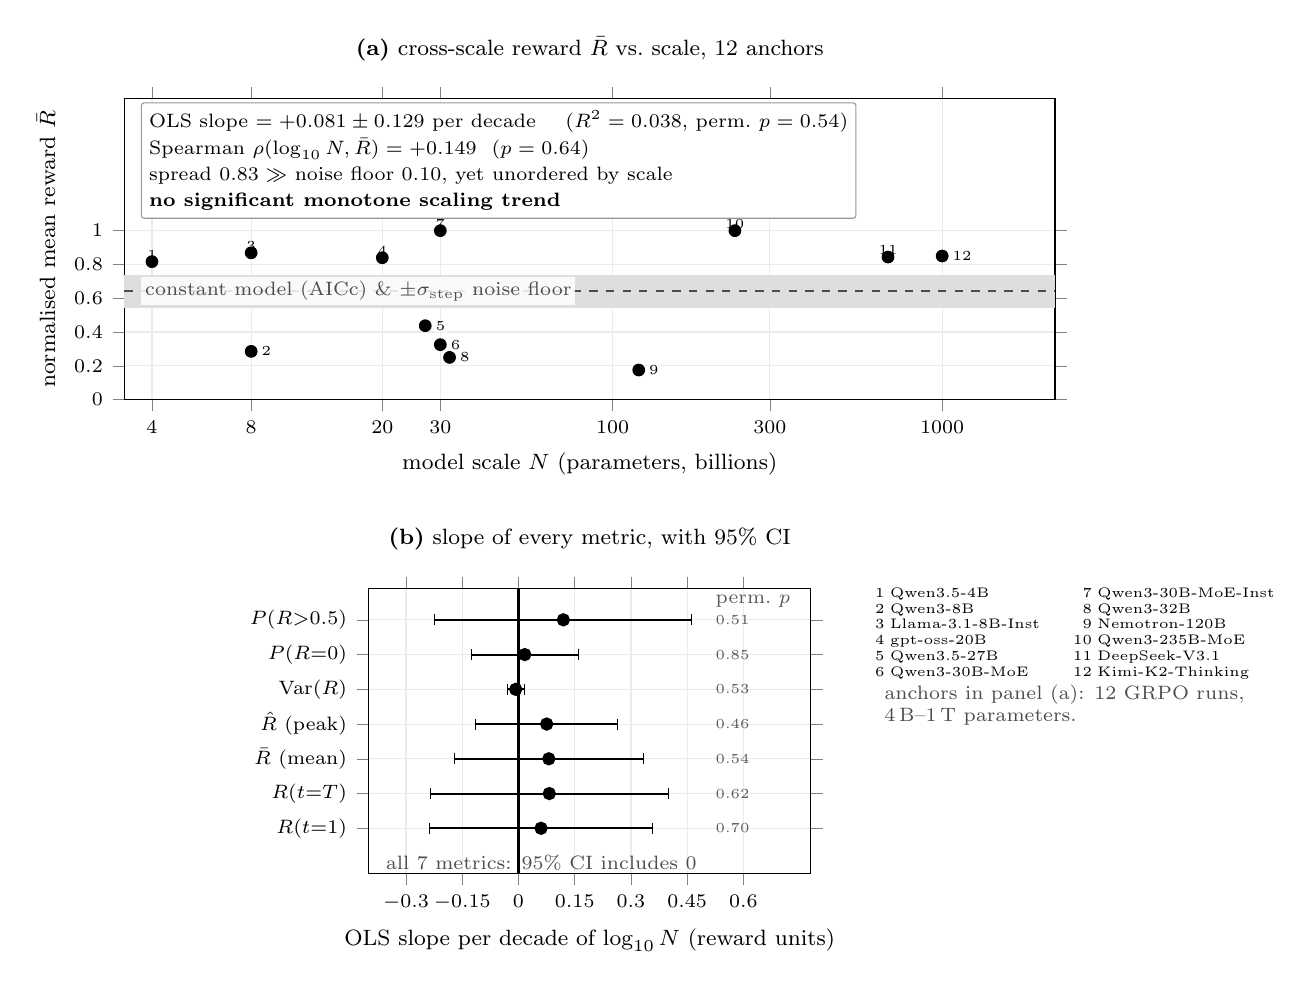
\begin{tikzpicture}
\begin{groupplot}[
  group style={group size=1 by 2, vertical sep=2.4cm},
  tick align=outside,
]

% ===================== PANEL (a): the cross-scale null =====================
\nextgroupplot[
  width=13.4cm, height=5.4cm,
  xmode=log,
  xmin=3.3, xmax=2200,
  ymin=0.0, ymax=1.78,
  xtick={4,8,20,30,100,300,1000},
  xticklabels={4,8,20,30,100,300,1000},
  xticklabel style={font=\scriptsize, /pgf/number format/fixed},
  ytick={0,0.2,0.4,0.6,0.8,1.0},
  yticklabel style={font=\scriptsize, /pgf/number format/fixed},
  xlabel={\footnotesize model scale $N$ (parameters, billions)},
  ylabel={\footnotesize normalised mean reward $\bar R$},
  title={\footnotesize\textbf{(a)} cross-scale reward $\bar R$ vs.\ scale, 12 anchors},
  title style={yshift=1.5mm},
  grid=major, grid style={black!8},
  clip=false,
]

% noise-floor band about the pooled mean (0.641): the measurement floor,
% NOT a trend.  Half-width = mean reported sigma_step (0.096).
\fill[black!13] (axis cs:3.3,0.5448) rectangle (axis cs:2200,0.7372);
% constant (intercept-only) model -- the AICc-selected best fit (iters 9/25)
\draw[black!70, thick, dashed] (axis cs:3.3,0.6410) -- (axis cs:2200,0.6410);

\addplot[only marks, mark=*, mark size=2.1pt, color=black] coordinates {
  (4,0.8167) (8,0.2854) (8,0.8688) (20,0.8396) (27,0.4373) (30,0.3252)
  (30,1.0000) (32,0.2497) (120,0.1750) (235,1.0000) (685,0.8438) (1000,0.8500)
};

% numbered tags -- numbers, not names, keep the plot free of label collisions
\node[tag, anchor=south]            at (axis cs:4,0.8167)    {1};
\node[tag, anchor=west, xshift=3pt] at (axis cs:8,0.2854)    {2};
\node[tag, anchor=south]            at (axis cs:8,0.8688)    {3};
\node[tag, anchor=south]            at (axis cs:20,0.8396)   {4};
\node[tag, anchor=west, xshift=3pt] at (axis cs:27,0.4373)   {5};
\node[tag, anchor=west, xshift=3pt] at (axis cs:30,0.3252)   {6};
\node[tag, anchor=south]            at (axis cs:30,1.0000)   {7};
\node[tag, anchor=west, xshift=3pt] at (axis cs:32,0.2497)   {8};
\node[tag, anchor=west, xshift=3pt] at (axis cs:120,0.1750)  {9};
\node[tag, anchor=south]            at (axis cs:235,1.0000)  {10};
\node[tag, anchor=south]            at (axis cs:685,0.8438)  {11};
\node[tag, anchor=west, xshift=3pt] at (axis cs:1000,0.8500) {12};

% --- the null, stated numerically (inside the figure) ---
\node[draw=black!40, thin, fill=white, rounded corners=1pt,
      align=left, font=\scriptsize, inner sep=2.8pt,
      anchor=north west] at (axis cs:3.7,1.76)
     {OLS slope $= +0.081 \pm 0.129$ per decade \quad ($R^{2}=0.038$, perm.\ $p=0.54$)\\[1.5pt]
      Spearman $\rho(\log_{10}N,\bar R) = +0.149$ \ ($p=0.64$)\\[1.5pt]
      spread $0.83 \gg$ noise floor $0.10$, yet unordered by scale\\[1.5pt]
      \textbf{no significant monotone scaling trend}};

% --- band / constant-model label, inside the axes at the left ---
\node[font=\scriptsize, text=black!70, fill=white, fill opacity=0.85,
      text opacity=1, inner sep=1.4pt, anchor=west]
     at (axis cs:3.7,0.6410)
     {constant model (AICc) \& $\pm\sigma_{\mathrm{step}}$ noise floor};

% ===================== PANEL (b): slope forest =====================
\nextgroupplot[
  width=7.2cm, height=5.2cm,
  xmin=-0.40, xmax=0.78,
  ymin=-1.3, ymax=6.9,
  ytick={0,1,2,3,4,5,6},
  yticklabels={$R(t{=}1)$,$R(t{=}T)$,$\bar R$ (mean),$\hat R$ (peak),
               $\mathrm{Var}(R)$,$P(R{=}0)$,$P(R{>}0.5)$},
  yticklabel style={font=\scriptsize},
  xtick={-0.3,-0.15,0,0.15,0.3,0.45,0.6},
  xticklabel style={font=\scriptsize, /pgf/number format/fixed},
  xlabel={\footnotesize OLS slope per decade of $\log_{10}N$ (reward units)},
  title={\footnotesize\textbf{(b)} slope of every metric, with 95\% CI},
  title style={yshift=1.5mm},
  grid=major, grid style={black!8},
  clip=false,
]
% zero reference
\draw[black, thick] (axis cs:0,-1.3) -- (axis cs:0,6.9);
\addplot[only marks, mark=*, mark size=2.0pt, color=black, thick,
         error bars/.cd, x dir=both, x explicit,
         error bar style={line width=0.7pt, draw=black}] coordinates {
  (0.0602,0) +- (0.2973,0)
  (0.0822,1) +- (0.3175,0)
  (0.0809,2) +- (0.2524,0)
  (0.0752,3) +- (0.1888,0)
  (-0.0074,4) +- (0.0223,0)
  (0.0167,5) +- (0.1431,0)
  (0.1197,6) +- (0.3426,0)
};
% permutation p-values (12 anchors) and column header
\node[font=\scriptsize, text=black!65, anchor=west] at (axis cs:0.50,6.55) {perm.\ $p$};
\node[font=\tiny,       text=black!65, anchor=west] at (axis cs:0.50,0) {0.70};
\node[font=\tiny,       text=black!65, anchor=west] at (axis cs:0.50,1) {0.62};
\node[font=\tiny,       text=black!65, anchor=west] at (axis cs:0.50,2) {0.54};
\node[font=\tiny,       text=black!65, anchor=west] at (axis cs:0.50,3) {0.46};
\node[font=\tiny,       text=black!65, anchor=west] at (axis cs:0.50,4) {0.53};
\node[font=\tiny,       text=black!65, anchor=west] at (axis cs:0.50,5) {0.85};
\node[font=\tiny,       text=black!65, anchor=west] at (axis cs:0.50,6) {0.51};
% the null statement, inside the axes clear of the last row (y = 0)
\node[font=\scriptsize, text=black!70, anchor=north west, align=left]
     at (axis cs:-0.38,-0.50)
     {all 7 metrics: 95\% CI includes $0$};

% --- anchor key, in the free space to the right of panel (b) ---
\node[keyfont, align=left, inner sep=0pt, anchor=west]
     at (axis cs:0.95,5.6)
     {\begin{tabular}{@{}r@{\hspace{2pt}}l@{\hspace{12pt}}r@{\hspace{2pt}}l@{}}
        1 & Qwen3.5-4B        & 7 & Qwen3-30B-MoE-Inst \\
        2 & Qwen3-8B          & 8 & Qwen3-32B \\
        3 & Llama-3.1-8B-Inst & 9 & Nemotron-120B \\
        4 & gpt-oss-20B       & 10 & Qwen3-235B-MoE \\
        5 & Qwen3.5-27B       & 11 & DeepSeek-V3.1 \\
        6 & Qwen3-30B-MoE     & 12 & Kimi-K2-Thinking \\
      \end{tabular}};
\node[font=\scriptsize, text=black!70, anchor=north west, align=left]
     at (axis cs:0.95,4.4)
     {anchors in panel (a): 12 GRPO runs,\\
      4\,B--1\,T parameters.};

\end{groupplot}
\end{tikzpicture}
\end{document}
